% Author: Izaak Neutelings (September 2020)
\documentclass[border=3pt,tikz]{standalone}
\usepackage{amsmath}
\usepackage{tikz}
\usepackage{physics}
\usepackage[outline]{contour} % glow around text
\usetikzlibrary{intersections}
\usetikzlibrary{decorations.markings}
\usetikzlibrary{angles,quotes} % for pic
\contourlength{1.2pt}

\tikzset{>=latex} % for LaTeX arrow head
\usepackage{xcolor}
\colorlet{veccol}{green!70!black}
\colorlet{vcol}{green!70!black}
\colorlet{xcol}{blue!85!black}
\colorlet{projcol}{xcol!60}
\colorlet{unitcol}{xcol!60!black!85}
\colorlet{myblue}{blue!70!black}
\colorlet{myred}{red!90!black}
\colorlet{mypurple}{blue!50!red!80!black!80}
\tikzstyle{vector}=[->,very thick,xcol]


\begin{document}


% VECTOR breakdown on axis
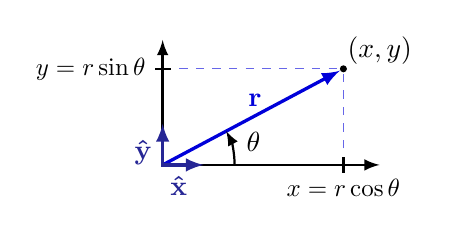
\begin{tikzpicture}
  \def\ul{0.52}
  \def\R{2.6}
  \def\ang{28}
  \coordinate (O) at (0,0);
  \coordinate (R) at (\ang:\R);
  \coordinate (X) at ({\R*cos(\ang)},0);
  \coordinate (Y) at (0,{\R*sin(\ang)});
  \node[fill=black,circle,inner sep=0.9] (R') at (R) {};
  \node[above right=-2] at (R') {$(x,y)$};
  \draw[<->,line width=0.9] %very thick
    ({1.2*\R*cos(\ang)},0) -- (O) -- (0,{1.3*\R*sin(\ang)});
  \draw[projcol,dashed] (X) -- (R);
  \draw[projcol,dashed] (Y) -- (R);
  \draw[vector] (O) -- (R') node[midway,left=5,above right=0] {$\vb{r}$};
  \draw[vector,<->,unitcol]
    (\ul,0) node[scale=1,left=2,below left=0] {$\vu{x}$} -- (O) --
    (0,\ul) node[scale=1,below=2,below left=0] {$\vu{y}$};
  \draw pic[->,thick,"$\theta$",draw=black,angle radius=26,angle eccentricity=1.3]
    {angle = X--O--R};
  \draw[thick] (X)++(0,0.1) --++ (0,-0.2) node[scale=0.9,below=-1] {$x = r\cos\theta$};
  \draw[thick] (Y)++(0.1,0) --++ (-0.2,0) node[scale=0.9,left] {$y = r\sin\theta$};
\end{tikzpicture}


% VECTOR breakdown in vectors
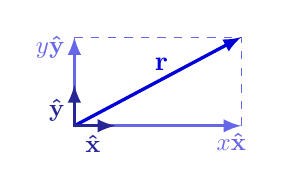
\begin{tikzpicture}
  \def\ul{0.52}
  \def\R{2.4}
  \def\ang{28}
  \coordinate (O) at (0,0);
  \coordinate (R) at (\ang:\R);
  \coordinate (X) at ({\R*cos(\ang)},0);
  \coordinate (Y) at (0,{\R*sin(\ang)});
  \draw[projcol,dashed] (X) -- (R);
  \draw[projcol,dashed] (Y) -- (R);
  \draw[vector] (O) -- (R) node[midway,left=5,above right=0] {$\vb{r}$};
  \draw[vector,<->,projcol]
    (X) node[scale=0.9,left=4,below=-1] {$x\vu{x}$} -- (O) --
    (Y) node[scale=0.9,below=4,left] {$y\vu{y}$};
  \draw[vector,<->,unitcol]
    (\ul,0) node[scale=0.9,left=2,below left=0] {$\vu{x}$} -- (O) --
    (0,\ul) node[scale=0.9,below=2,below left=0] {$\vu{y}$};
  %\draw pic[->,thick,"$\theta$",draw=black,angle radius=26,angle eccentricity=1.3]
  %  {angle = X--O--R};
\end{tikzpicture}


% VECTOR breakdown - all
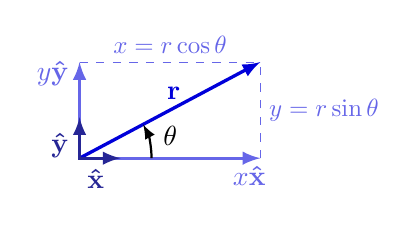
\begin{tikzpicture}
  \def\ul{0.52}
  \def\R{2.6}
  \def\ang{28}
  \coordinate (O) at (0,0);
  \coordinate (R) at (\ang:\R);
  \coordinate (X) at ({\R*cos(\ang)},0);
  \coordinate (Y) at (0,{\R*sin(\ang)});
  \draw[projcol,dashed] (X) -- (R) node[scale=0.9,midway,right] {$y = r\sin\theta$};
  \draw[projcol,dashed] (Y) -- (R) node[scale=0.9,midway,above] {$x = r\cos\theta$};
  \draw[vector] (O) -- (R) node[midway,left=5,above right=0] {$\vb{r}$};
  \draw[vector,<->,projcol]
    (X) node[scale=1,left=4,below=-1] {$x\vu{x}$} -- (O) --
    (Y) node[scale=1,below=4,left] {$y\vu{y}$};
  \draw[vector,<->,unitcol]
    (\ul,0) node[scale=1,left=2,below left=0] {$\vu{x}$} -- (O) --
    (0,\ul) node[scale=1,below=2,below left=0] {$\vu{y}$};
  \draw pic[->,thick,"$\theta$",draw=black,angle radius=26,angle eccentricity=1.3]
    {angle = X--O--R};
\end{tikzpicture}


% VECTOR breakdown - all - velocity
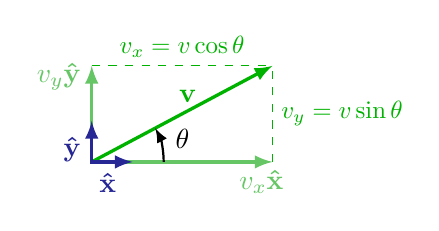
\begin{tikzpicture}
  \def\ul{0.52}
  \def\R{2.6}
  \def\ang{28}
  \coordinate (O) at (0,0);
  \coordinate (R) at (\ang:\R);
  \coordinate (X) at ({\R*cos(\ang)},0);
  \coordinate (Y) at (0,{\R*sin(\ang)});
  \draw[projcol,dashed,veccol] (X) -- (R) node[scale=0.9,midway,right] {$v_y = v\sin\theta$};
  \draw[projcol,dashed,veccol] (Y) -- (R) node[scale=0.9,midway,above] {$v_x = v\cos\theta$};
  \draw[vector,vcol] (O) -- (R) node[midway,left=5,above right=0] {$\vb{v}$};
  \draw[vector,<->,vcol!90!black!60]
    (X) node[scale=1,left=4,below=-1] {$v_x\vu{x}$} -- (O) --
    (Y) node[scale=1,below=4,left] {$v_y\vu{y}$};
  \draw[vector,<->,unitcol]
    (\ul,0) node[scale=1,left=2,below left=0] {$\vu{x}$} -- (O) --
    (0,\ul) node[scale=1,below=2,below left=0] {$\vu{y}$};
  \draw pic[->,thick,"$\theta$",draw=black,angle radius=26,angle eccentricity=1.3]
    {angle = X--O--R};
\end{tikzpicture}


% VECTOR scaling
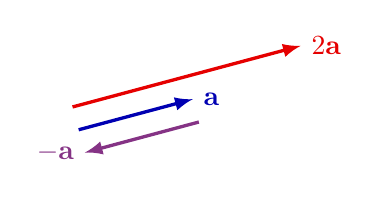
\begin{tikzpicture}
  \def\ul{0.52}
  \def\R{1.5}
  \def\ang{15}
  \draw[vector,myblue]
    (0,0) -- (\ang:\R) node[right=0] {$\vb{a}$};
  \draw[vector,mypurple,shift={(\ang-90:0.3)}]
    (\ang:\R) -- (0,0) node[above=0,left=0] {$-\vb{a}$};
  \draw[vector,myred,shift={(\ang+90:0.3)}]
    (0,0) -- (\ang:2*\R) node[right=0] {$2\vb{a}$};
\end{tikzpicture}


% VECTOR projection
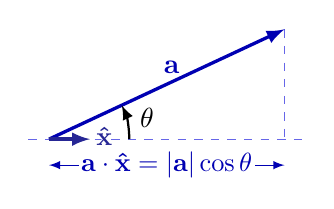
\begin{tikzpicture}
  \def\ul{0.52}
  \def\R{3.3}
  \def\ang{25}
  \coordinate (O) at (0,0);
  \coordinate (R) at (\ang:\R);
  \coordinate (X) at ({\R*cos(\ang)},0);
  \draw[projcol,dashed] (R) -- (X);
  \draw[projcol,dashed] (-0.08*\R,0) -- (X) --++ (0.08*\R,0);
  \draw[vector,myblue] (O) -- (R) node[midway,left=5,above right=0] {$\vb{a}$};
  %\draw[vector,veccol!70]
  %  (O) -- (X) node[scale=0.8,left=4,below=-1] {$(\vb{r}\cdot\vu{x})\vu{x} = (r\cos\theta)\vu{x}$};
  %\node[myblue,scale=0.8,left=4,below=-1] at (X) {$\vb{a}\cdot\vu{x} = \abs{\vb{a}}\cos\theta$};
  \draw[myblue,<->]
    (O)++(0,-0.1*\R) --++ ({\R*cos(\ang)},0)
    node[scale=0.95,midway,fill=white,inner sep=1] {$\vb{a}\cdot\vu{x} = \abs{\vb{a}}\cos\theta$};
  \draw[vector,unitcol]
    (O) -- (\ul,0) node[scale=0.95,above=1,right=-1.5] {\contour{white}{$\vu{x}$}}; %,below left=0
  \draw pic[->,thick,"$\theta$",draw=black,angle radius=29,angle eccentricity=1.25]
    {angle = X--O--R};
\end{tikzpicture}


% VECTOR projection
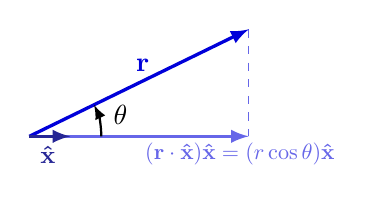
\begin{tikzpicture}
  \def\ul{0.52}
  \def\R{3.1}
  \def\ang{26}
  \coordinate (O) at (0,0);
  \coordinate (R) at (\ang:\R);
  \coordinate (X) at ({\R*cos(\ang)},0);
  \draw[projcol,dashed] (R) -- (X);
  \draw[vector] (O) -- (R) node[midway,left=5,above right=0] {$\vb{r}$};
  \draw[vector,projcol]
    (O) -- (X) node[scale=0.8,left=4,below=-1] {$(\vb{r}\cdot\vu{x})\vu{x} = (r\cos\theta)\vu{x}$};
  \draw[vector,unitcol]
    (O) -- (\ul,0) node[scale=0.9,left=2,below left=0] {$\vu{x}$};
  \draw pic[->,thick,"$\theta$",draw=black,angle radius=26,angle eccentricity=1.3]
    {angle = X--O--R};
\end{tikzpicture}


%% VECTOR projection
%\begin{tikzpicture}
%  \def\A{2.0}
%  \def\B{2.9}
%  \def\ang{34}
%  \coordinate (O) at (0,0);
%  \coordinate (A) at (\ang:\A);
%  \coordinate (B) at (\B,0);
%  \coordinate (Ax) at ({\A*cos(\ang)},0);
%  \draw[projcol,dashed] (A) -- (Ax);
%  \draw[vector,red!90!black] (O) -- (A) node[above right=-2] {$\vb{a}$};
%  \draw[vector,blue!90!black] (O) -- (B) node[right=-1] {$\vb{b}$};
%  \draw[vector,blue!50!red!80] (O) -- (Ax) node[midway,below] {$\vb{a}\cdot\vb{b}$};
%\end{tikzpicture}




\end{document}